\chapter{根轨迹法}

\intro{根轨迹法是W. R. Evans于1948年提出的一种图解法，用于分析闭环系统极点随增益参数变化的轨迹。它不需复杂的代数运算即可直观揭示系统动态特性随参数的变化规律。}

\section{根轨迹的基本概念}

\subsection{问题的提出}

给定反馈系统，前向通道传递函数为$KG(s)$，反馈通道为$H(s)$，其中$K \geq 0$为可调增益。闭环特征方程为：
\[
1 + KG(s)H(s) = 0
\]
等价于：
\[
KG(s)H(s) = -1
\]

当$K$从$0$变化到$+\infty$时，闭环特征方程的根（即闭环极点）在复平面上描绘出的轨迹称为\textbf{根轨迹}。

\begin{mydefinition}{根轨迹（Root Locus）}
根轨迹是闭环系统特征方程的根（闭环极点）在复平面上随某一参数（通常为开环增益$K$）从$0$变化至$+\infty$时形成的轨迹曲线。根轨迹始于开环极点（$K=0$），终于开环零点（$K\to\infty$）。
\end{mydefinition}

根轨迹法的核心价值在于：\textbf{开环的零极点分布已知，即可绘制闭环极点轨迹，进而分析闭环系统的稳定性、动态品质和稳态误差}，而无需直接求解高阶特征方程。

\subsection{开环传递函数与闭环极点的关系}

将开环传递函数写为零极点形式：
\[
G(s)H(s) = \frac{N(s)}{D(s)} = K^* \frac{\prod_{i=1}^{m} (s-z_i)}{\prod_{j=1}^{n} (s-p_j)}
\]
其中$K^*$为根轨迹增益，$z_i$为开环零点，$p_j$为开环极点。根轨迹方程为：
\[
1 + K^* \frac{\prod_{i=1}^{m} (s-z_i)}{\prod_{j=1}^{n} (s-p_j)} = 0
\]
即：
\[
\prod_{j=1}^{n} (s-p_j) + K^* \prod_{i=1}^{m} (s-z_i) = 0
\]

当$K^* = 0$时，方程退化为$\prod_{j=1}^{n} (s-p_j) = 0$，闭环极点为开环极点$p_j$。当$K^* \to \infty$时，方程退化为$\prod_{i=1}^{m} (s-z_i) = 0$，闭环极点趋于开环零点$z_i$。若$n > m$（物理系统通常如此），则有$(n-m)$条根轨迹分支趋于无穷远。

\section{幅值条件与相角条件}

根轨迹方程$KG(s)H(s) = -1$可分解为两个等价条件：

\begin{myformula}
\textbf{根轨迹的幅值条件与相角条件：}
\text{幅值条件:}&\quad |KG(s)H(s)| = 1,\quad\text{即}\quad K = \frac{1}{|G(s)H(s)|} \\
\text{相角条件:}&\quad \angle G(s)H(s) = \pm (2k+1)\pi,\quad k=0,1,2,\dots
\end{myformula}

\begin{proof}[相角条件的推导]
$KG(s)H(s) = -1 = 1 \cdot e^{j(2k+1)\pi}$，故$\angle [KG(s)H(s)] = \angle G(s)H(s) = (2k+1)\pi$（增益$K$为正实数，辐角为0）。
\end{proof}

相角条件是判定复平面上某点$s$是否在根轨迹上的判据——它\textbf{不依赖于}增益$K$。幅值条件则用于确定根轨迹上的$s$点对应的$K$值。

用零极点形式表达：
\begin{itemize}
\item 相角条件：$\sum_{i=1}^{m} \angle(s - z_i) - \sum_{j=1}^{n} \angle(s - p_j) = (2k+1)\pi$
\item 幅值条件：$K^* = \frac{\prod_{j=1}^{n} |s - p_j|}{\prod_{i=1}^{m} |s - z_i|}$
\end{itemize}

\begin{figure}[H]
\centering
\begin{tikzpicture}[scale=1.2,
    ctrlAxRL/.style={->,>=stealth,thick},
    ctrlPointRL/.style={fill=black,circle,inner sep=1.5pt},
    ctrlZeroRL/.style={fill=white,draw=black,circle,inner sep=1.5pt,thick},
    ctrlLineRL/.style={dashed,blue!60,->,>=stealth},
]
\draw[ctrlAxRL] (-0.5,0) -- (6,0) node[right] {$\sigma$};
\draw[ctrlAxRL] (0,-2.5) -- (0,2.5) node[above] {$j\omega$};
% Test point s
\node[ctrlPointRL,label={[font=\footnotesize]above right:$s$}] at (3.5, 1.5) {};
% Pole p1
\node[ctrlPointRL,label={[font=\footnotesize]below right:$p_1$}] at (1.0, -1.5) {};
\node[ctrlPointRL,label={[font=\footnotesize]above right:$p_2$}] at (1.0, 1.5) {};
% Zero z1
\node[ctrlZeroRL,label={[font=\footnotesize]below left:$z_1$}] at (5.0, -0.5) {};
% Vectors from poles to s
\draw[ctrlLineRL] (1.0, -1.5) -- (3.5, 1.5) node[midway,below,font=\footnotesize] {$\vec{s}-p_1$};
\draw[ctrlLineRL] (1.0, 1.5) -- (3.5, 1.5) node[midway,above,font=\footnotesize] {$\vec{s}-p_2$};
% Vector from zero to s
\draw[ctrlLineRL] (5.0, -0.5) -- (3.5, 1.5) node[midway,above right,font=\tiny] {$\vec{s}-z_1$};
% Angle annotations
\draw[->] (1.8, -0.3) arc[start angle=-30, end angle=50, radius=0.6];
\node[font=\footnotesize] at (2.2, -0.2) {$\theta_1$};
\draw[->] (2.2, 1.2) arc[start angle=60, end angle=0, radius=0.6];
\node[font=\footnotesize] at (2.6, 1.3) {$\theta_2$};
\draw[->] (4.5, 0.2) arc[start angle=-100, end angle=-150, radius=0.6];
\node[font=\footnotesize] at (4.4, -0.5) {$\phi_1$};
% Formula
\node[font=\footnotesize, align=center] at (3.0, -2.3) {$\theta_1+\theta_2-\phi_1 = (2k+1)\pi$};
\end{tikzpicture}
\caption{相角条件的几何解释：从各极点/零点指向试探点$s$的向量辐角之和满足$(2k+1)\pi$}
\label{fig:angle-condition}
\end{figure}

\section{根轨迹的绘制规则}

基于相角条件和幅值条件，W. R. Evans于1948年总结了10条根轨迹绘制规则。掌握这些规则即可快速、准确地勾画根轨迹的大致形状和走向。

\begin{myalgorithm}{根轨迹的10条绘制规则（Evans法则）}
\begin{enumerate}
\item \textbf{起点与终点}：根轨迹有$n$条分支。$K^*=0$时各分支从开环极点$p_j$出发；$K^*\to\infty$时$m$条分支终止于开环零点$z_i$，剩余$(n-m)$条分支沿渐近线趋于无穷远。

\item \textbf{分支数、连续性与对称性}：根轨迹有$n = \max(n,m)$条分支；各分支是$K^*$的连续曲线；且关于实轴对称（因为特征方程为实系数方程）。

\item \textbf{实轴上的根轨迹}：实轴上某区域属于根轨迹的充要条件是——该区域右侧的开环实极点和实零点的总个数为奇数。

\textbf{证明}：实轴上任意试探点$s$，所有共轭复数和实轴上左侧的零极点对其提供的相角代数和为0；只有右侧的实极点和实零点中每个提供$+\pi$或$-\pi$（取决于方向）。因此右侧奇数个点时总相角为奇数倍$\pi$，满足相角条件。

\item \textbf{渐近线}：$(n-m)$条趋于无穷的分支沿$(n-m)$条渐近线趋近。渐近线与实轴的交点$\sigma_a$和夹角$\phi_a$为：
\[
\sigma_a = \frac{\sum_{j=1}^{n} p_j - \sum_{i=1}^{m} z_i}{n-m}, \qquad
\phi_a = \frac{(2k+1)\pi}{n-m}, \quad k=0,1,\dots,n-m-1
\]

\item \textbf{分离点（会合点）}：两条或以上根轨迹分支在实轴上相遇后又分开的点。分离点$s_b$满足：
\[
\sum_{j=1}^{n} \frac{1}{s_b - p_j} = \sum_{i=1}^{m} \frac{1}{s_b - z_i}
\]
等价于$\frac{d}{ds}\left[\frac{D(s)}{N(s)}\right] = 0$或$\frac{dK^*}{ds} = 0$。

\item \textbf{出射角（从复极点出发的角度）与入射角（进入复零点的角度）}：
从复极点$p_\ell$的出射角：
\[
\theta_{p_\ell} = 180^\circ - \sum_{j\neq\ell} \angle(p_\ell-p_j) + \sum_{i=1}^{m} \angle(p_\ell-z_i)
\]
进入复零点$z_\ell$的入射角：
\[
\phi_{z_\ell} = 180^\circ + \sum_{j=1}^{n} \angle(z_\ell-p_j) - \sum_{i\neq\ell} \angle(z_\ell-z_i)
\]

\item \textbf{虚轴交点}：根轨迹与虚轴的交点$s = j\omega$可通过两种方法求得：(a) 令特征方程$1+G(j\omega)H(j\omega)=0$，即$\Re[1+GH] = 0$且$\Im[1+GH] = 0$，联立求解$\omega$和$K^*$；(b) 用Routh判据确定临界增益。

\item \textbf{根之和}：当$n-m \geq 2$时，闭环极点之和等于开环极点之和（与$K^*$无关）：
\[
\sum_{j=1}^{n} \lambda_j = \sum_{j=1}^{n} p_j = \text{常数}
\]
这一性质意味着此时闭环极点组的重心在复平面上的位置不随增益变化——某条分支向左移动必然伴随着另一分支向右移动。

\item \textbf{根之积}：闭环极点之积与开环增益有关：
\[
\prod_{j=1}^{n} |\lambda_j| = \left|\prod_{j=1}^{n} p_j + K^* \prod_{i=1}^{m} z_i\right|
\]

\item \textbf{增益$K^*$的确定}：根轨迹上任意点$s_x$对应的增益值由幅值条件给出：
\[
K^* = \frac{\prod_{j=1}^{n} |s_x - p_j|}{\prod_{i=1}^{m} |s_x - z_i|}
\]
\end{enumerate}
\end{myalgorithm}

\begin{remark}
这10条规则中，规则1（起点终点）、规则3（实轴分布）、规则4（渐近线）、规则5（分离点）、规则6（出射入射角）和规则7（虚轴交点）是绘制准确根轨迹的关键。规则8（根之和）和规则9（根之积）主要用于验证和简化计算。规则2（对称性）总是成立。
\end{remark}

\subsection{绘制规则的应用示例——二阶系统}

考虑开环传递函数：
\[
G(s)H(s) = \frac{K}{s(s+a)}, \quad a > 0
\]

\textbf{步骤1：} 开环极点$p_1 = 0$，$p_2 = -a$；无有限零点；$n=2, m=0$。

\textbf{步骤2：} $n-m = 2$条渐近线。
\[
\sigma_a = \frac{0 + (-a) - 0}{2} = -\frac{a}{2}, \quad
\phi_a = \frac{(2k+1)\pi}{2} = \frac{\pi}{2},\ \frac{3\pi}{2}
\]
即渐近线为过点$(-a/2, 0)$的两条垂直线。

\textbf{步骤3：} 实轴分布：$[-a, 0]$段在根轨迹上（该段右侧有2个极点——偶数？等等，仔细算：在$[-a,0]$段内，右侧有$p_1=0$——1个，奇数个，所以在轨迹上）。正确：区间$(-\infty, -a]$右侧2个极点（偶数），不在轨迹上；区间$[-a, 0]$右侧1个极点（奇数），在轨迹上；区间$[0, \infty)$右侧0个，不在轨迹上。

\textbf{步骤4：} 分离点：由规则5，
\[
\frac{1}{s_b} + \frac{1}{s_b + a} = 0 \implies 2s_b + a = 0 \implies s_b = -\frac{a}{2}
\]
分离角为$\pm90^\circ$（两分支对称离开实轴）。

\textbf{步骤5：} 根轨迹：始于$0$和$-a$，沿实轴相向运动，在$-a/2$汇合后以$\pm90^\circ$角度垂直离开实轴，沿渐近线趋于无穷。该轨迹是\textbf{垂直于实轴}通过$(-a/2,0)$的直线。

\begin{figure}[H]
\centering
\begin{tikzpicture}[scale=1.1,
    ctrlAx2/.style={->,>=stealth,thick},
    ctrlRL/.style={thick, blue!60},
    ctrlPole/.style={fill=blue!60,circle,inner sep=2pt},
    ctrlBran/.style={->,>=stealth,thick,blue!60},
]
\draw[ctrlAx2] (-4,0) -- (1.5,0) node[right] {$\sigma$};
\draw[ctrlAx2] (0,-3) -- (0,3) node[above] {$j\omega$};
% Poles
\node[ctrlPole,label={[font=\footnotesize]below:$p_1=0$}] (P1) at (0,0) {};
\node[ctrlPole,label={[font=\footnotesize]below:$p_2=-a$}] (P2) at (-3,0) {};
% Breakaway point
\node[fill=green!50!black,circle,inner sep=1.5pt] at (-1.5,0) {};
\node[font=\footnotesize] at (-1.5,-0.4) {$-\frac{a}{2}$};
% Root locus branches
\draw[ctrlRL] (0,0) -- (-1.5,0);
\draw[ctrlRL] (-3,0) -- (-1.5,0);
\draw[ctrlBran] (-1.5,0) -- (-1.5, 2.8);
\draw[ctrlBran] (-1.5,0) -- (-1.5, -2.8);
% Asymptote
\node[font=\footnotesize,rotate=90] at (-2.2, 2.2) {渐近线 $\sigma_a=-\frac{a}{2}$};
\draw[dashed,gray!60] (-1.5, -3) -- (-1.5, 3);
\end{tikzpicture}
\caption{二阶系统$G(s)=K/[s(s+a)]$的根轨迹}
\label{fig:root-locus-2nd}
\end{figure}

此系统具有重要的物理意义：\textbf{无论$K$取何正值，闭环极点始终具有负实部，系统总是稳定的}。当$K$增大时，阻尼比$\zeta$减小，响应振荡加剧，但系统始终稳定——这是二阶系统的固有特性，也是"二阶系统无条件稳定"这一结论在根轨迹中的直观体现。

\subsection{三阶系统的根轨迹}

考虑$G(s)H(s) = \frac{K}{s(s+1)(s+2)}$。

开环极点$p_1=0$，$p_2=-1$，$p_3=-2$；$n=3, m=0$。

\textbf{渐近线：} $n-m=3$。
\[
\sigma_a = \frac{0-1-2}{3} = -1, \quad
\phi_a = \frac{\pi}{3},\ \pi,\ \frac{5\pi}{3} \quad (60^\circ, 180^\circ, 300^\circ)
\]

\textbf{实轴分布：} $[-1,0]$段和$(-\infty,-2]$段在轨迹上。

\textbf{分离点：}
\[
\frac{1}{s} + \frac{1}{s+1} + \frac{1}{s+2} = 0 \implies 3s^2 + 6s + 2 = 0
\]
解得$s_{b1} \approx -0.423$（在$[-1,0]$内），$s_{b2} \approx -1.577$。$-1.577$不在实轴根轨迹段内（$[-2,-1]$段不在轨迹上），故仅$s_{b1} \approx -0.423$为有效分离点。

\textbf{虚轴交点：} 特征方程$s^3+3s^2+2s+K=0$。构造Routh表：
\[
\begin{array}{c|cc}
s^3: & 1 & 2 \\
s^2: & 3 & K \\
s^1: & \frac{6-K}{3} & 0 \\
s^0: & K &
\end{array}
\]
令$s^1$行第一列$(6-K)/3 = 0$，得临界增益$K_c = 6$。辅助方程$3s^2+K=0$，代入$K=6$：$3s^2+6=0$，$s = \pm j\sqrt{2}$。

\textbf{结论：} 当$0 < K < 6$时系统稳定；当$K=6$时临界稳定（纯虚极点$\pm j\sqrt{2}$）；当$K>6$时系统不稳定（两条分支进入右半平面）。

\begin{figure}[H]
\centering
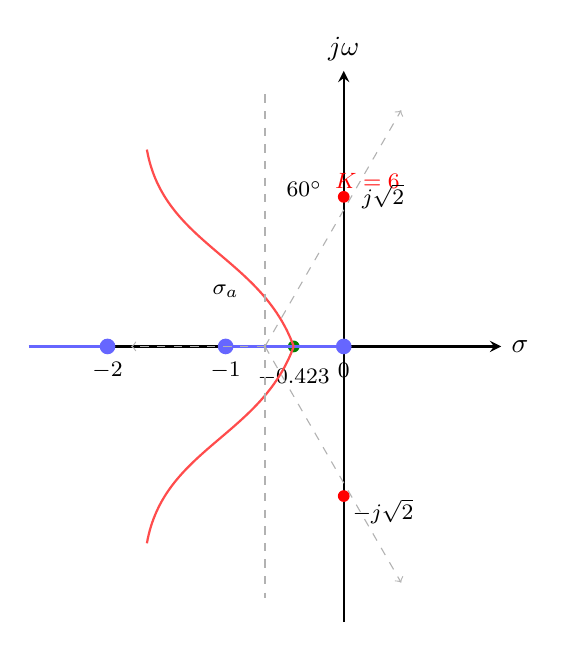
\begin{tikzpicture}[scale=1.0,
    ctrlAx3/.style={->,>=stealth,thick},
    ctrlRL3/.style={thick,blue!60},
    ctrlRL3B/.style={thick,red!70},
    ctrlPole3/.style={fill=blue!60,circle,inner sep=2pt},
]
\draw[ctrlAx3] (-4,0) -- (2,0) node[right] {$\sigma$};
\draw[ctrlAx3] (0,-3.5) -- (0,3.5) node[above] {$j\omega$};
% Poles
\node[ctrlPole3] (P0) at (0,0) {};
\node[ctrlPole3] (P1) at (-1.5,0) {};
\node[ctrlPole3] (P2) at (-3,0) {};
\node[font=\footnotesize] at (0,-0.3) {$0$};
\node[font=\footnotesize] at (-1.5,-0.3) {$-1$};
\node[font=\footnotesize] at (-3,-0.3) {$-2$};
% Breakaway
\node[fill=green!50!black,circle,inner sep=1.5pt] at (-0.635,0) {};
\node[font=\footnotesize] at (-0.635,-0.4) {$-0.423$};
% Branches on real axis
\draw[ctrlRL3] (0,0) -- (-0.635,0);
\draw[ctrlRL3] (-1.5,0) -- (-0.635,0);
\draw[ctrlRL3] (-3,0) -- (-4,0);
% Complex branches (approximate curves)
\draw[ctrlRL3B] (-0.635,0) to[out=110,in=-80] (-2.5,2.5);
\draw[ctrlRL3B] (-0.635,0) to[out=-110,in=80] (-2.5,-2.5);
% Asymptotes
\draw[dashed,gray!60] (-1,3.2) -- (-1,0) -- (-1,-3.2);
\node[font=\footnotesize] at (-1.5,0.7) {$\sigma_a$};
\draw[dashed,gray!60,->] (-1,0) -- (-1+1.73,3.0);
\draw[dashed,gray!60,->] (-1,0) -- (-2.7,0);
\draw[dashed,gray!60,->] (-1,0) -- (-1+1.73,-3.0);
\node[font=\footnotesize] at (-0.5,2.0) {$60^\circ$};
% Imag axis intersection
\node[fill=red,circle,inner sep=1.5pt] at (0,1.9) {};
\node[fill=red,circle,inner sep=1.5pt] at (0,-1.9) {};
\node[font=\footnotesize,red] at (0.3,2.1) {$K=6$};
\node[font=\footnotesize] at (0.5,1.9) {$j\sqrt{2}$};
\node[font=\footnotesize] at (0.5,-2.1) {$-j\sqrt{2}$};
\end{tikzpicture}
\caption{三阶系统$G(s)=K/[s(s+1)(s+2)]$的根轨迹}
\label{fig:root-locus-3rd}
\end{figure}

\subsection*{Python示例：用Python绘制根轨迹}

\newpage

\begin{lstlisting}[language=Python]
import numpy as np
import matplotlib.pyplot as plt
from scipy import signal

def plot_root_locus(num, den, K_range=None):
    """绘制根轨迹（简易版：对K采样求闭环极点）"""
    if K_range is None:
        K_range = np.logspace(-2, 2, 500)

    poles_all = []
    for K in K_range:
        # 闭环特征多项式: den(s) + K * num(s)
        # 注意: num和den必须同长，不足补0
        n = max(len(num), len(den))
        num_pad = np.hstack([np.zeros(n - len(num)), num])
        den_pad = np.hstack([np.zeros(n - len(den)), den])
        closed_den = den_pad + K * num_pad
        poles = np.roots(closed_den)
        poles_all.append(poles)

    poles_all = np.array(poles_all)

    plt.figure(figsize=(10, 8))
    # 绘制各极点随K变化的轨迹
    for j in range(poles_all.shape[1]):
        plt.plot(np.real(poles_all[:, j]), 
                 np.imag(poles_all[:, j]), 'b.', markersize=1)

    # 标注开环极点和零点
    open_poles = np.roots(den)
    open_zeros = np.roots(num)
    plt.plot(np.real(open_poles), np.imag(open_poles), 
             'rx', markersize=10, markeredgewidth=2, label='开环极点')
    if len(open_zeros) > 0:
        plt.plot(np.real(open_zeros), np.imag(open_zeros), 
                 'go', markersize=10, label='开环零点')

    plt.axhline(y=0, color='k', linewidth=0.5)
    plt.axvline(x=0, color='k', linewidth=0.5)
    plt.xlabel('实轴 $\\sigma$')
    plt.ylabel('虚轴 $j\\omega$')
    plt.title('根轨迹图')
    plt.legend()
    plt.grid(True, alpha=0.3)
    plt.axis('equal')
    plt.show()

# 示例: G(s)H(s) = K / [s(s+1)(s+2)]
num = [1]
den = [1, 3, 2, 0]
plot_root_locus(num, den, K_range=np.logspace(-2, 1.2, 800))
\end{lstlisting}

\section{参数根轨迹}

\subsection{非增益参数变化的根轨迹}

有时需要分析除开环增益$K$以外的其他参数变化对系统性能的影响。以$G(s)H(s) = \frac{10}{s(s+T)}$为例，分析时间常数$T$从$0$到$\infty$变化时的根轨迹。

此时特征方程为$s^2 + Ts + 10 = 0$。将含$T$的项移到分子：
\[
1 + T \cdot \frac{s}{s^2 + 10} = 0
\]
等效开环传递函数为$G_{\text{eq}}(s) = \frac{s}{s^2+10}$，$T$为"等效增益"。开环极点$p_{1,2} = \pm j\sqrt{10}$，开环零点$z_1 = 0$。

$n=2, m=1$，渐近线：$\sigma_a = \frac{0-0}{1} = 0$（实际上在此例中确切形式需要具体分析...更准确地：原特征方程为$s^2 + Ts + 10 = 0$，即$s = \frac{-T \pm \sqrt{T^2 - 40}}{2}$）。当$T < 2\sqrt{10} \approx 6.32$时系统欠阻尼；$T = 6.32$时临界阻尼；$T > 6.32$时过阻尼。

\begin{remark}
参数根轨迹表明：标准根轨迹的10条规则同样适用于非增益参数$\alpha$的根轨迹，只需将特征方程改写为$1 + \alpha \cdot G_{\text{eq}}(s) = 0$的形式即可，其中$\alpha$为待分析参数。
\end{remark}

\section{基于根轨迹的系统性能分析}

\subsection{主导极点概念}

\begin{mydefinition}{主导极点}
闭环系统中，那些距离虚轴最近且附近无闭环零点的极点称为主导极点。高阶系统的动态响应主要由其主导极点决定——远离虚轴的极点对应的暂态分量衰减极为迅速，对系统响应的贡献可忽略。
\end{mydefinition}

\begin{figure}[H]
\centering
\begin{tikzpicture}[scale=1.0,
    ctrlAxD/.style={->,>=stealth,thick},
]
\draw[ctrlAxD] (-6,0) -- (1,0) node[right] {$\sigma$};
\draw[ctrlAxD] (0,-4) -- (0,4) node[above] {$j\omega$};
% Dominant poles (closest to jw axis)
\node[fill=blue!60,circle,inner sep=2.5pt] (D1) at (-0.8, 1.8) {};
\node[fill=blue!60,circle,inner sep=2.5pt] (D2) at (-0.8, -1.8) {};
\node[font=\footnotesize,blue!60] at (-0.5, 2.1) {主导极点};
\node[font=\footnotesize,blue!60] at (-0.5, -2.3) {主导极点};
% Far poles
\node[fill=gray!50,circle,inner sep=2pt] at (-4.5, 0.8) {};
\node[fill=gray!50,circle,inner sep=2pt] at (-4.5, -0.8) {};
\node[fill=gray!50,circle,inner sep=2pt] at (-5.2, 1.6) {};
\node[fill=gray!50,circle,inner sep=2pt] at (-5.2, -1.6) {};
\node[font=\footnotesize,gray!50] at (-4.5, -1.3) {非主导极点};
% Dominant region
\draw[dashed,red!60] (-1.5,-2.5) -- (-1.5,2.5);
\node[font=\footnotesize,red!60] at (-1.5,2.8) {主导区域分界线};
% Zero
\node[fill=white,draw=black,circle,inner sep=2pt] (Z1) at (-1.5,0) {};
\node[font=\footnotesize] at (-1.2,-0.4) {零点（靠近主导极点时影响显著）};
\end{tikzpicture}
\caption{主导极点概念示意}
\label{fig:dominant-poles}
\end{figure}

若主导极点为$s_{1,2} = -\zeta\omega_n \pm j\omega_n\sqrt{1-\zeta^2}$，则系统近似为二阶系统，其时域性能可由前面章节的公式直接估算。主导极点判别准则：距虚轴的距离至少为其他极点的$1/5$（即非主导极点实部至少为主导极点实部的$5$倍）。

\subsection{附加极点对系统性能的影响}

\textbf{附加极点使系统响应变慢}。在原开环系统中加入一个实极点$-p$（$p>0$）：根轨迹向右弯曲，导致主导极点的阻尼比减小（振荡加剧）、实部绝对值减小（响应变慢）。从物理角度看，附加极点引入了额外的"惯性"，使系统响应迟钝。

\textbf{附加闭环极点使稳定性裕度减小}。这一点在根轨迹上表现为主导极点向虚轴方向偏移，临界增益降低。

\subsection{附加零点对系统性能的影响}

\textbf{附加零点使系统响应加快}。加入一个实零点$-z$：根轨迹向左弯曲，主导极点向远离虚轴方向运动，阻尼比增大。但当零点位置过于靠右时可能使系统不稳定。

\begin{remark}
附加零极点对系统动态品质的影响可总结为：{\heiti 左极点使响应变慢，左零点使响应加快}。这是控制系统中一种深刻的对偶关系，反映了传递函数零极点配置与系统动态之间的内在联系。
\end{remark}

\section{基于根轨迹的补偿设计}

根轨迹法不仅可用于分析，更可用于设计与综合。基本思路是：若系统的根轨迹不满足性能指标，则在系统中引入附加零极点（即串联补偿器），改变根轨迹的形状，使其通过期望的闭环极点位置。

\subsection{超前补偿（相位超前网络）}

超前补偿器的传递函数为：
\[
G_c(s) = K_c \frac{s + z_c}{s + p_c}, \quad |z_c| < |p_c|
\]
零点靠近虚轴（或位于期望区域），极点远离虚轴。其效果是"吸引"根轨迹向左移动，增加系统阻尼和带宽。

\subsection{滞后补偿（相位滞后网络）}

滞后补偿器的传递函数为：
\[
G_c(s) = K_c \frac{s + z_c}{s + p_c}, \quad |p_c| < |z_c|
\]
极点和零点靠得很近且紧邻原点，用于提高稳态精度（增大低频增益）而不显著改变暂态响应。

\subsection{设计流程}

\begin{myalgorithm}{基于根轨迹的补偿器设计步骤}
\begin{enumerate}
\item 根据时域性能指标（$\sigma\%$、$t_s$）确定期望的闭环主导极点位置$s_{1,2} = -\zeta\omega_n \pm j\omega_n\sqrt{1-\zeta^2}$。
\item 绘制原系统根轨迹，检查是否经过期望极点区域。若是，则仅需调节增益$K$；若否，则需要加入补偿器。
\item 选择补偿器类型（超前/滞后/超前-滞后），确定零极点位置。
\item 由相角条件和幅值条件计算补偿器参数和系统增益。
\item 验证补偿后系统的时域响应，必要时迭代调整。
\end{enumerate}
\end{myalgorithm}

\subsection*{Python示例：补偿器设计与根轨迹验证}

\begin{lstlisting}[language=Python]
import numpy as np
import control as ct

# 被控对象：Gp(s) = 1 / [s(s+1)]
num_p = [1]
den_p = [1, 1, 0]
Gp = ct.tf(num_p, den_p)

# 期望性能: zeta >= 0.5, ts(2%) <= 4s
# -> zeta*wn >= 1 -> wn >= 2
# 期望主导极点: s_d = -zeta*wn +/- j*wn*sqrt(1-zeta^2)
zeta_d = 0.5
wn_d = 2.0
wd = wn_d * np.sqrt(1 - zeta_d**2)
s_d = complex(-zeta_d * wn_d, wd)
print(f"期望闭环主导极点: s_d = {s_d:.4f}")

# 求原系统在期望极点处的相位缺额
val = ct.evalfr(Gp, s_d)
phase_deficiency = np.pi - np.angle(val)
print(f"相位缺额: {np.degrees(phase_deficiency):.2f} deg")

# 设计超前补偿器（此处仅示意，实际需完整设计算法）
# 补偿器形式: Gc(s) = Kc * (s+z_c)/(s+p_c)
# ...（详细设计代码见后续频域章节）

# 验证补偿后系统
# G_ol = Gc * Gp
# rlocus(G_ol) 检查是否通过期望极点
\end{lstlisting}

\section*{本章小结}

根轨迹法是经典控制理论中最重要的图解分析方法之一。它将闭环极点在复平面上的运动轨迹可视化，为系统分析与综合提供了直观、有力的工具。本章从根轨迹的基本概念出发，详细阐述了相角条件和幅值条件这两个基础等式，系统整理了Evans的10条绘制规则，并通过二阶与三阶系统的典型实例演示了规则的应用。主导极点概念为高阶系统的降阶近似分析提供了理论依据。最后，根轨迹补偿设计作为分析与综合的连接桥梁，展示了根轨迹法在实际控制工程中的价值。
